\section{Motivation}
\label{sec:motivation}

\begin{figure}[!t]
\centering
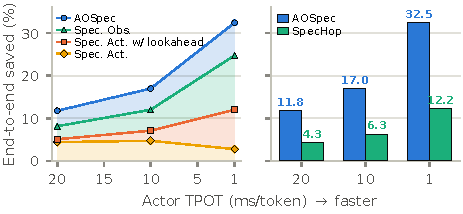
\includegraphics[width=\columnwidth]{figs/tool_share}
\caption{End-to-end latency savings under trace replay, averaged over nine
(harness, model) configurations on Terminal Bench. Left: ceiling gaps among the Spec. Act, Spec. Act w/ lookahead, Spec. Obs, and
\sysname{}. Right: \sysname{} versus SpecHop at 20/10/1\,ms per token.}
\label{fig:tpot}
\end{figure}

We model a disaggregated agent as an actor and an environment runtime. At step $i$, the actor takes $\dtime_i$ time to generate action $a_i$, and the runtime takes $\ttime_i$ time to execute it and return observation $o_i$, yielding serial latency $\sum_i(\dtime_i+\ttime_i)$. Observation speculation drafts $\hat{o}_i$ so the actor can advance while $a_i$ executes. 
Action speculation drafts and begins executing $\hat{a}_i$ before $a_i$ is emitted. 
By profiling 1{,}921 training-set trajectories across nine Terminal Bench harness--model configurations~\citep{terminalbench2},
we identify three fundamental challenges: latency concentration, environment-dependent observations, and the tension between longer overlap and compounding chain-prediction error.

\begin{figure*}[!t]
\centering
\begingroup
\newlength{\motivationpanelheight}
\setlength{\motivationpanelheight}{0.150\textwidth}
\newcommand{\motivationpanel}[3]{%
  \begin{minipage}[t]{#1}
    \centering
    \vspace{0pt}% anchor every panel at the same top edge
    \parbox[t][\motivationpanelheight][t]{\linewidth}{%
      \centering
      \includegraphics[
        width=\linewidth,
        height=\motivationpanelheight,
        keepaspectratio
      ]{#2}%
    }%
    \par\vspace{0.15em}
    \footnotesize\bfseries #3
  \end{minipage}%
}
\motivationpanel{0.232\textwidth}{figs/concentration}{(a) Concentration}\hfill
\motivationpanel{0.220\textwidth}{figs/latency_scatter}{(b) Latency scatter}\hfill
\motivationpanel{0.300\textwidth}{figs/obs.pdf}{(c) Qualitative examples}\hfill
\motivationpanel{0.233\textwidth}{figs/lookahead}{(d) Overlap ceiling}
\endgroup
\caption{Motivating measurements from Terminal Bench.
(a) A small fraction of long calls accounts for almost all tool time.
(b) Per-step latency spans both model-bound and tool-bound regimes.
(c) Qualitative examples of costly environment-dependent observations.
(d) Longer lookahead raises the oracle overlap ceiling, but empirical exact-chain
hit rate collapses.}
\label{fig:motivation}
\end{figure*}

\subsection{Latency Concentration Decouples Hits from Savings}
\label{sec:challenge1}

As shown in Figure~\ref{fig:motivation}(a), tool time of computer-using agents is highly concentrated: the 17\% of calls lasting at least one second account for 97\% of total tool time.
Figure~\ref{fig:motivation}(b) shows the same mismatch at the step level: execution spans both model-bound and tool-bound regimes, so equal hit counts need not hide equal amounts of time.
A predictor correct only on these long-running calls would hide 97\% of tool time by achieving only 17\% hit rate. 
Conversely, a predictor correct on all remaining calls would achieve an 83\% hit rate but hide only 3\%. Thus, hit rate alone poorly reflects speculative latency savings.

\insightbox{\textbf{Insight 1:} Speculation value is concentrated: predicting
a few slow calls can hide nearly all tool time.}

\subsection{Environment Dependence Limits Observation Prediction}
\label{sec:challenge2}

Observation speculation is limited by the information available in the
actor's context. Figure~\ref{fig:motivation}(c) contrasts a predictable
file-comparison result with training metrics revealed only through execution.
More broadly, many latency-critical observations depend on hidden environment
state, such as files, running processes, or available resources, and therefore
cannot be predicted reliably from the actor's context alone.

For observations beyond this information boundary, executing a predicted
action early can supply the missing result, but only conditionally. 
Since a mispredicted action may corrupt the environment, speculative execution
can safely complement observation prediction only when contained in a sandbox
that supports snapshotting and forking.

\insightbox{\textbf{Insight 2:} Environment-dependent outcomes demand execution, not prediction: sandboxed action speculation reveals them early without risking committed state.}

\subsection{Longer Lookahead Creates Runway but Collapses Prediction Accuracy}
\label{sec:challenge3}

A speculative action launched when its issuing decode begins can hide at most
$\min(\dtime_i,\ttime_i)$. As decoding accelerates, this runway shrinks:
Figure~\ref{fig:motivation}(d) shows that the one-step overlap ceiling falls
from 43.3\% to 25.7\% as per-token latency decreases from 20\,ms to 1\,ms.

Looking farther ahead restores the lost runway: at 1\,ms, increasing the
horizon from one to five steps raises the idealized ceiling from 25.7\% to
65.2\%. 
However, prior multi-step approaches require the entire predicted action chain to match~\citep{sui2026parallelizing,bpaste2026,ye2025speculative}, causing accuracy to
collapse multiplicatively from 20.9\% at one step to 2.4\% at three and 1.2\% at five. 
The speculative timing that offers the most runway is therefore the least likely to realize it.

\insightbox{\textbf{Insight 3:} Farther lookahead creates runway, but multiplicative chain errors erase the overlap it is meant to unlock.}

Together, these findings identify three barriers to useful speculation and motivate the design of \sysname{}.